%% prisma_flow.tex — Fluxograma PRISMA-ScR
%% Incluído via %% prisma_flow.tex — Fluxograma PRISMA-ScR
%% Incluído via %% prisma_flow.tex — Fluxograma PRISMA-ScR
%% Incluído via %% prisma_flow.tex — Fluxograma PRISMA-ScR
%% Incluído via \input{prisma_flow} no figure environment de main.tex
%% Valores marcados com [N] aguardam buscas institucionais (Murilo).
%% PubMed (8) = exato via API NCBI jun/2026; demais = estimados.

\usetikzlibrary{positioning, calc, arrows.meta}

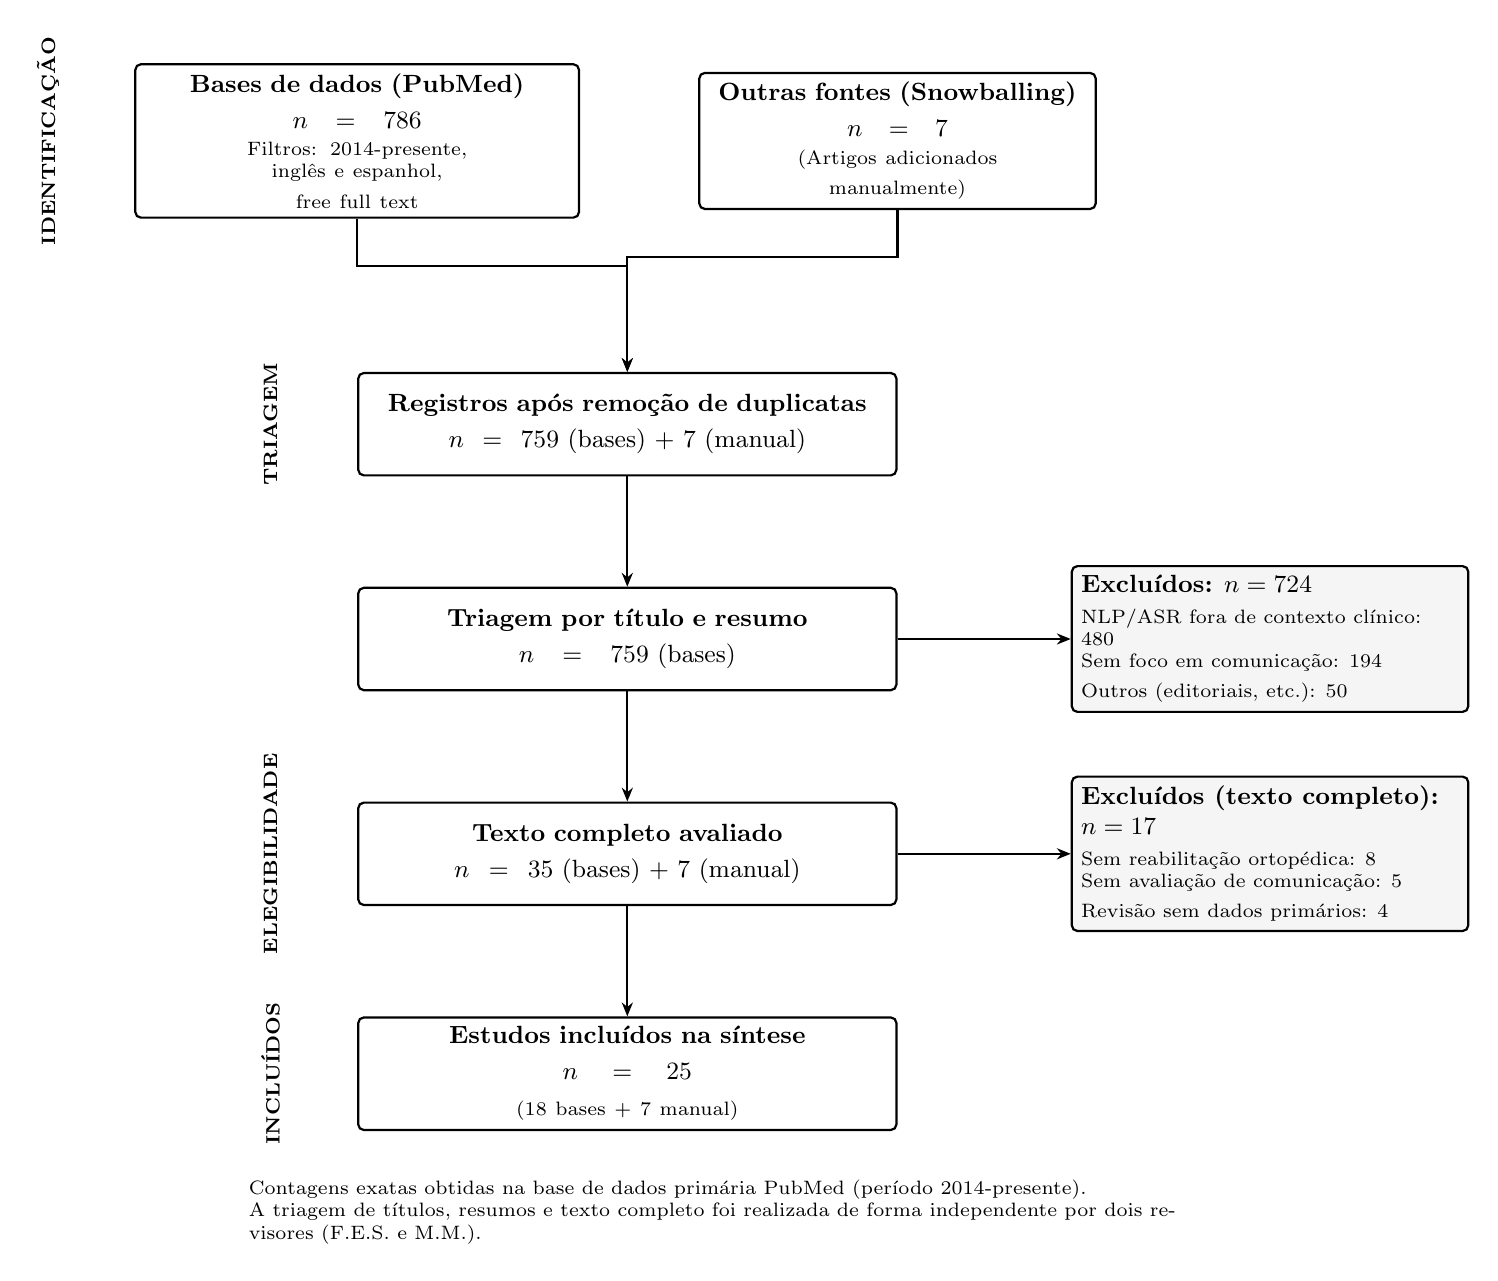
\begin{tikzpicture}[
  %% caixas do fluxo principal
  mbox/.style={
    rectangle, draw=black, thick, rounded corners=2pt,
    minimum width=6.8cm, text width=6.6cm,
    minimum height=1.3cm, align=center,
    fill=white, font=\small
  },
  %% caixas de exclusão (margem direita)
  ebox/.style={
    rectangle, draw=black, thick, rounded corners=2pt,
    minimum width=5.0cm, text width=4.8cm,
    minimum height=1.3cm, align=flush left,
    fill=gray!8, font=\small
  },
  %% setas
  arr/.style={-{Stealth[length=5pt,width=4pt]}, thick},
  %% labels de fase
  phase/.style={font=\bfseries\scriptsize, rotate=90, anchor=center}
]

%% ================================================================
%% ================================================================
%% FASE 1 — IDENTIFICAÇÃO
%% ================================================================
\node[mbox, minimum width=5.6cm, text width=5.4cm] (dbbox) at (-1.8, 0) {
  \textbf{Bases de dados (PubMed)}\\[2pt]
  $n = 786$\\[2pt]
  {\scriptsize Filtros: 2014-presente,\\
    inglês e espanhol,\\
    free full text}
};

\node[mbox, minimum width=5.0cm, text width=4.8cm,
      right=1.5cm of dbbox] (otherbox) {
  \textbf{Outras fontes (Snowballing)}\\[2pt]
  $n = 7$\\[2pt]
  {\scriptsize (Artigos adicionados\\
    manualmente)}
};

%% ================================================================
%% FASE 2 — TRIAGEM
%% ================================================================
%% Centro entre as duas caixas de identificação
\coordinate (midid) at ($(dbbox.south)!0.5!(otherbox.south)$);

\node[mbox, below=2.0cm of midid, anchor=north] (dedup) {
  \textbf{Registros após remoção de duplicatas}\\[2pt]
  $n = 759$ (bases) + $7$ (manual)
};

%% setas de convergência
\draw[arr] (dbbox.south)  -- ++(0,-0.6cm) -| (dedup.north);
\draw[arr] (otherbox.south) -- ++(0,-0.6cm) -| (dedup.north);

\node[mbox, below=1.4cm of dedup] (screen) {
  \textbf{Triagem por título e resumo}\\[2pt]
  $n = 759$ (bases)
};

\draw[arr] (dedup) -- (screen);

\node[ebox, right=2.2cm of screen] (excl1) {
  \textbf{Excluídos:} $n = 724$\\[3pt]
  {\scriptsize
    NLP/ASR fora de contexto clínico: 480\\
    Sem foco em comunicação: 194\\
    Outros (editoriais, etc.): 50
  }
};

\draw[arr] (screen.east) -- (excl1.west);

%% ================================================================
%% FASE 3 — ELEGIBILIDADE
%% ================================================================
\node[mbox, below=1.4cm of screen] (eligib) {
  \textbf{Texto completo avaliado}\\[2pt]
  $n = 35$ (bases) + $7$ (manual)
};

\draw[arr] (screen) -- (eligib);

\node[ebox, right=2.2cm of eligib] (excl2) {
  \textbf{Excluídos (texto completo):} $n = 17$\\[3pt]
  {\scriptsize
    Sem reabilitação ortopédica: 8\\
    Sem avaliação de comunicação: 5\\
    Revisão sem dados primários: 4
  }
};

\draw[arr] (eligib.east) -- (excl2.west);

%% ================================================================
%% FASE 4 — INCLUÍDOS
%% ================================================================
\node[mbox, below=1.4cm of eligib] (included) {
  \textbf{Estudos incluídos na síntese}\\[2pt]
  $n = 25$\\[2pt]
  {\scriptsize (18 bases + 7 manual)}
};

\draw[arr] (eligib) -- (included);

%% ================================================================
%% LABELS DE FASE (margem esquerda)
%% ================================================================
\node[phase] at ($(dbbox.west) + (-1.1cm, 0)$)      {IDENTIFICAÇÃO};
\node[phase] at ($(dedup.west)  + (-1.1cm, 0)$)      {TRIAGEM};
\node[phase] at ($(screen.west) + (-1.1cm, 0)$)      {};   %% continua triagem
\node[phase] at ($(eligib.west) + (-1.1cm, 0)$)      {ELEGIBILIDADE};
\node[phase] at ($(included.west) + (-1.1cm, 0)$)    {INCLUÍDOS};

%% ================================================================
%% NOTA DE RODAPÉ
%% ================================================================
\node[font=\scriptsize, anchor=north west, text width=12cm]
  at ($(included.south west) + (-1.5cm, -0.5cm)$) {%
  Contagens exatas obtidas na base de dados primária PubMed (período 2014-presente). \\
  A triagem de títulos, resumos e texto completo foi realizada de forma independente por dois revisores (F.E.S.\ e M.M.).
};

\end{tikzpicture} no figure environment de main.tex
%% Valores marcados com [N] aguardam buscas institucionais (Murilo).
%% PubMed (8) = exato via API NCBI jun/2026; demais = estimados.

\usetikzlibrary{positioning, calc, arrows.meta}

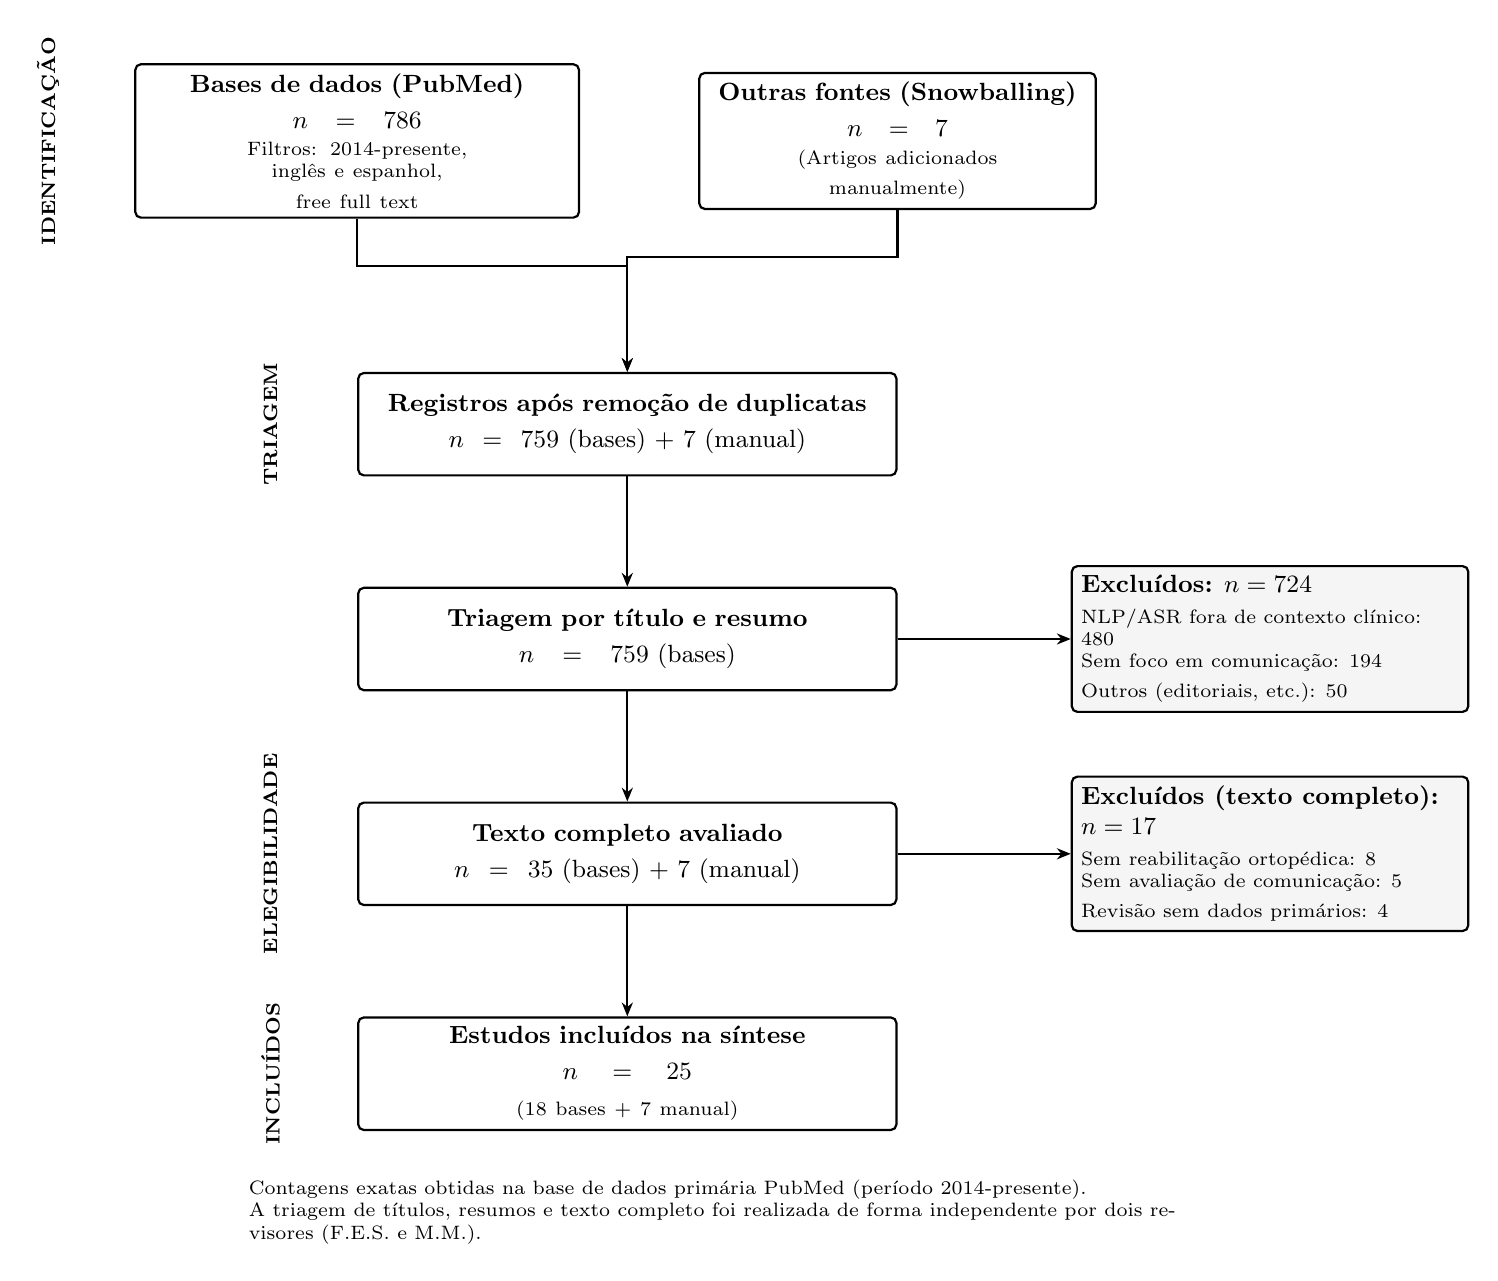
\begin{tikzpicture}[
  %% caixas do fluxo principal
  mbox/.style={
    rectangle, draw=black, thick, rounded corners=2pt,
    minimum width=6.8cm, text width=6.6cm,
    minimum height=1.3cm, align=center,
    fill=white, font=\small
  },
  %% caixas de exclusão (margem direita)
  ebox/.style={
    rectangle, draw=black, thick, rounded corners=2pt,
    minimum width=5.0cm, text width=4.8cm,
    minimum height=1.3cm, align=flush left,
    fill=gray!8, font=\small
  },
  %% setas
  arr/.style={-{Stealth[length=5pt,width=4pt]}, thick},
  %% labels de fase
  phase/.style={font=\bfseries\scriptsize, rotate=90, anchor=center}
]

%% ================================================================
%% ================================================================
%% FASE 1 — IDENTIFICAÇÃO
%% ================================================================
\node[mbox, minimum width=5.6cm, text width=5.4cm] (dbbox) at (-1.8, 0) {
  \textbf{Bases de dados (PubMed)}\\[2pt]
  $n = 786$\\[2pt]
  {\scriptsize Filtros: 2014-presente,\\
    inglês e espanhol,\\
    free full text}
};

\node[mbox, minimum width=5.0cm, text width=4.8cm,
      right=1.5cm of dbbox] (otherbox) {
  \textbf{Outras fontes (Snowballing)}\\[2pt]
  $n = 7$\\[2pt]
  {\scriptsize (Artigos adicionados\\
    manualmente)}
};

%% ================================================================
%% FASE 2 — TRIAGEM
%% ================================================================
%% Centro entre as duas caixas de identificação
\coordinate (midid) at ($(dbbox.south)!0.5!(otherbox.south)$);

\node[mbox, below=2.0cm of midid, anchor=north] (dedup) {
  \textbf{Registros após remoção de duplicatas}\\[2pt]
  $n = 759$ (bases) + $7$ (manual)
};

%% setas de convergência
\draw[arr] (dbbox.south)  -- ++(0,-0.6cm) -| (dedup.north);
\draw[arr] (otherbox.south) -- ++(0,-0.6cm) -| (dedup.north);

\node[mbox, below=1.4cm of dedup] (screen) {
  \textbf{Triagem por título e resumo}\\[2pt]
  $n = 759$ (bases)
};

\draw[arr] (dedup) -- (screen);

\node[ebox, right=2.2cm of screen] (excl1) {
  \textbf{Excluídos:} $n = 724$\\[3pt]
  {\scriptsize
    NLP/ASR fora de contexto clínico: 480\\
    Sem foco em comunicação: 194\\
    Outros (editoriais, etc.): 50
  }
};

\draw[arr] (screen.east) -- (excl1.west);

%% ================================================================
%% FASE 3 — ELEGIBILIDADE
%% ================================================================
\node[mbox, below=1.4cm of screen] (eligib) {
  \textbf{Texto completo avaliado}\\[2pt]
  $n = 35$ (bases) + $7$ (manual)
};

\draw[arr] (screen) -- (eligib);

\node[ebox, right=2.2cm of eligib] (excl2) {
  \textbf{Excluídos (texto completo):} $n = 17$\\[3pt]
  {\scriptsize
    Sem reabilitação ortopédica: 8\\
    Sem avaliação de comunicação: 5\\
    Revisão sem dados primários: 4
  }
};

\draw[arr] (eligib.east) -- (excl2.west);

%% ================================================================
%% FASE 4 — INCLUÍDOS
%% ================================================================
\node[mbox, below=1.4cm of eligib] (included) {
  \textbf{Estudos incluídos na síntese}\\[2pt]
  $n = 25$\\[2pt]
  {\scriptsize (18 bases + 7 manual)}
};

\draw[arr] (eligib) -- (included);

%% ================================================================
%% LABELS DE FASE (margem esquerda)
%% ================================================================
\node[phase] at ($(dbbox.west) + (-1.1cm, 0)$)      {IDENTIFICAÇÃO};
\node[phase] at ($(dedup.west)  + (-1.1cm, 0)$)      {TRIAGEM};
\node[phase] at ($(screen.west) + (-1.1cm, 0)$)      {};   %% continua triagem
\node[phase] at ($(eligib.west) + (-1.1cm, 0)$)      {ELEGIBILIDADE};
\node[phase] at ($(included.west) + (-1.1cm, 0)$)    {INCLUÍDOS};

%% ================================================================
%% NOTA DE RODAPÉ
%% ================================================================
\node[font=\scriptsize, anchor=north west, text width=12cm]
  at ($(included.south west) + (-1.5cm, -0.5cm)$) {%
  Contagens exatas obtidas na base de dados primária PubMed (período 2014-presente). \\
  A triagem de títulos, resumos e texto completo foi realizada de forma independente por dois revisores (F.E.S.\ e M.M.).
};

\end{tikzpicture} no figure environment de main.tex
%% Valores marcados com [N] aguardam buscas institucionais (Murilo).
%% PubMed (8) = exato via API NCBI jun/2026; demais = estimados.

\usetikzlibrary{positioning, calc, arrows.meta}

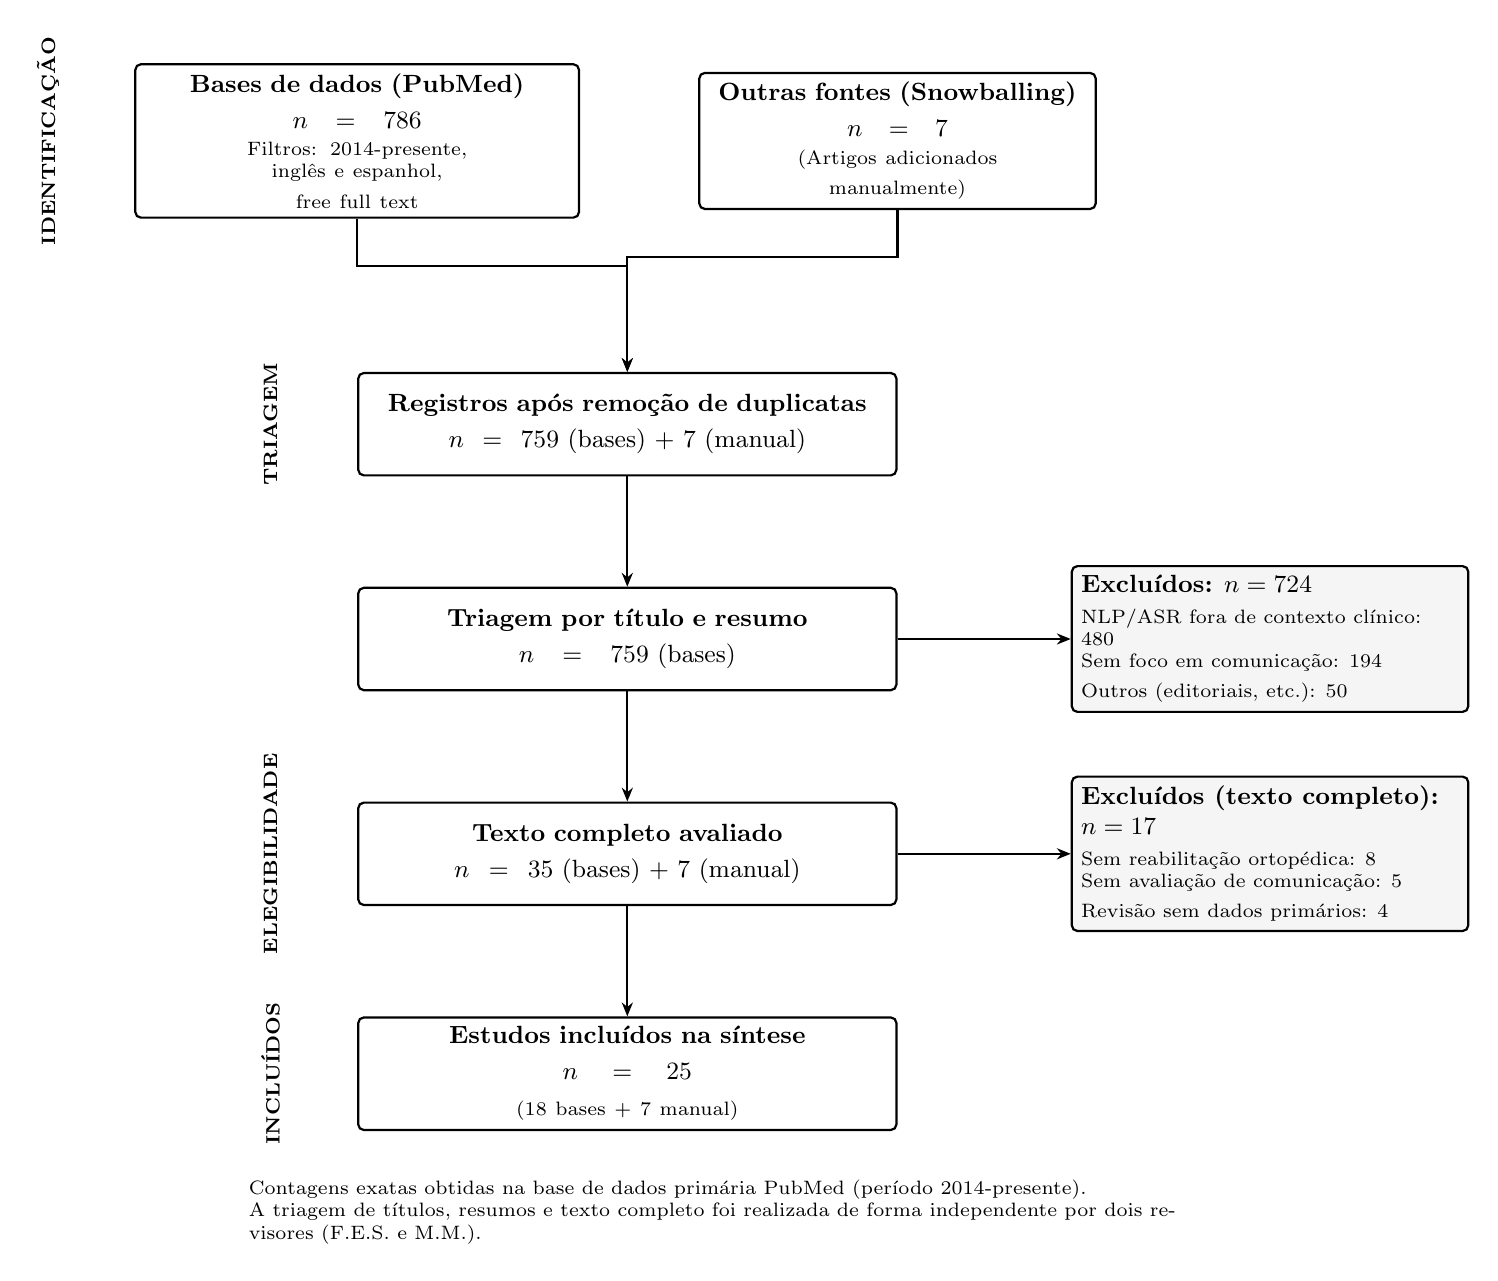
\begin{tikzpicture}[
  %% caixas do fluxo principal
  mbox/.style={
    rectangle, draw=black, thick, rounded corners=2pt,
    minimum width=6.8cm, text width=6.6cm,
    minimum height=1.3cm, align=center,
    fill=white, font=\small
  },
  %% caixas de exclusão (margem direita)
  ebox/.style={
    rectangle, draw=black, thick, rounded corners=2pt,
    minimum width=5.0cm, text width=4.8cm,
    minimum height=1.3cm, align=flush left,
    fill=gray!8, font=\small
  },
  %% setas
  arr/.style={-{Stealth[length=5pt,width=4pt]}, thick},
  %% labels de fase
  phase/.style={font=\bfseries\scriptsize, rotate=90, anchor=center}
]

%% ================================================================
%% ================================================================
%% FASE 1 — IDENTIFICAÇÃO
%% ================================================================
\node[mbox, minimum width=5.6cm, text width=5.4cm] (dbbox) at (-1.8, 0) {
  \textbf{Bases de dados (PubMed)}\\[2pt]
  $n = 786$\\[2pt]
  {\scriptsize Filtros: 2014-presente,\\
    inglês e espanhol,\\
    free full text}
};

\node[mbox, minimum width=5.0cm, text width=4.8cm,
      right=1.5cm of dbbox] (otherbox) {
  \textbf{Outras fontes (Snowballing)}\\[2pt]
  $n = 7$\\[2pt]
  {\scriptsize (Artigos adicionados\\
    manualmente)}
};

%% ================================================================
%% FASE 2 — TRIAGEM
%% ================================================================
%% Centro entre as duas caixas de identificação
\coordinate (midid) at ($(dbbox.south)!0.5!(otherbox.south)$);

\node[mbox, below=2.0cm of midid, anchor=north] (dedup) {
  \textbf{Registros após remoção de duplicatas}\\[2pt]
  $n = 759$ (bases) + $7$ (manual)
};

%% setas de convergência
\draw[arr] (dbbox.south)  -- ++(0,-0.6cm) -| (dedup.north);
\draw[arr] (otherbox.south) -- ++(0,-0.6cm) -| (dedup.north);

\node[mbox, below=1.4cm of dedup] (screen) {
  \textbf{Triagem por título e resumo}\\[2pt]
  $n = 759$ (bases)
};

\draw[arr] (dedup) -- (screen);

\node[ebox, right=2.2cm of screen] (excl1) {
  \textbf{Excluídos:} $n = 724$\\[3pt]
  {\scriptsize
    NLP/ASR fora de contexto clínico: 480\\
    Sem foco em comunicação: 194\\
    Outros (editoriais, etc.): 50
  }
};

\draw[arr] (screen.east) -- (excl1.west);

%% ================================================================
%% FASE 3 — ELEGIBILIDADE
%% ================================================================
\node[mbox, below=1.4cm of screen] (eligib) {
  \textbf{Texto completo avaliado}\\[2pt]
  $n = 35$ (bases) + $7$ (manual)
};

\draw[arr] (screen) -- (eligib);

\node[ebox, right=2.2cm of eligib] (excl2) {
  \textbf{Excluídos (texto completo):} $n = 17$\\[3pt]
  {\scriptsize
    Sem reabilitação ortopédica: 8\\
    Sem avaliação de comunicação: 5\\
    Revisão sem dados primários: 4
  }
};

\draw[arr] (eligib.east) -- (excl2.west);

%% ================================================================
%% FASE 4 — INCLUÍDOS
%% ================================================================
\node[mbox, below=1.4cm of eligib] (included) {
  \textbf{Estudos incluídos na síntese}\\[2pt]
  $n = 25$\\[2pt]
  {\scriptsize (18 bases + 7 manual)}
};

\draw[arr] (eligib) -- (included);

%% ================================================================
%% LABELS DE FASE (margem esquerda)
%% ================================================================
\node[phase] at ($(dbbox.west) + (-1.1cm, 0)$)      {IDENTIFICAÇÃO};
\node[phase] at ($(dedup.west)  + (-1.1cm, 0)$)      {TRIAGEM};
\node[phase] at ($(screen.west) + (-1.1cm, 0)$)      {};   %% continua triagem
\node[phase] at ($(eligib.west) + (-1.1cm, 0)$)      {ELEGIBILIDADE};
\node[phase] at ($(included.west) + (-1.1cm, 0)$)    {INCLUÍDOS};

%% ================================================================
%% NOTA DE RODAPÉ
%% ================================================================
\node[font=\scriptsize, anchor=north west, text width=12cm]
  at ($(included.south west) + (-1.5cm, -0.5cm)$) {%
  Contagens exatas obtidas na base de dados primária PubMed (período 2014-presente). \\
  A triagem de títulos, resumos e texto completo foi realizada de forma independente por dois revisores (F.E.S.\ e M.M.).
};

\end{tikzpicture} no figure environment de main.tex
%% Valores marcados com [N] aguardam buscas institucionais (Murilo).
%% PubMed (8) = exato via API NCBI jun/2026; demais = estimados.

\usetikzlibrary{positioning, calc, arrows.meta}

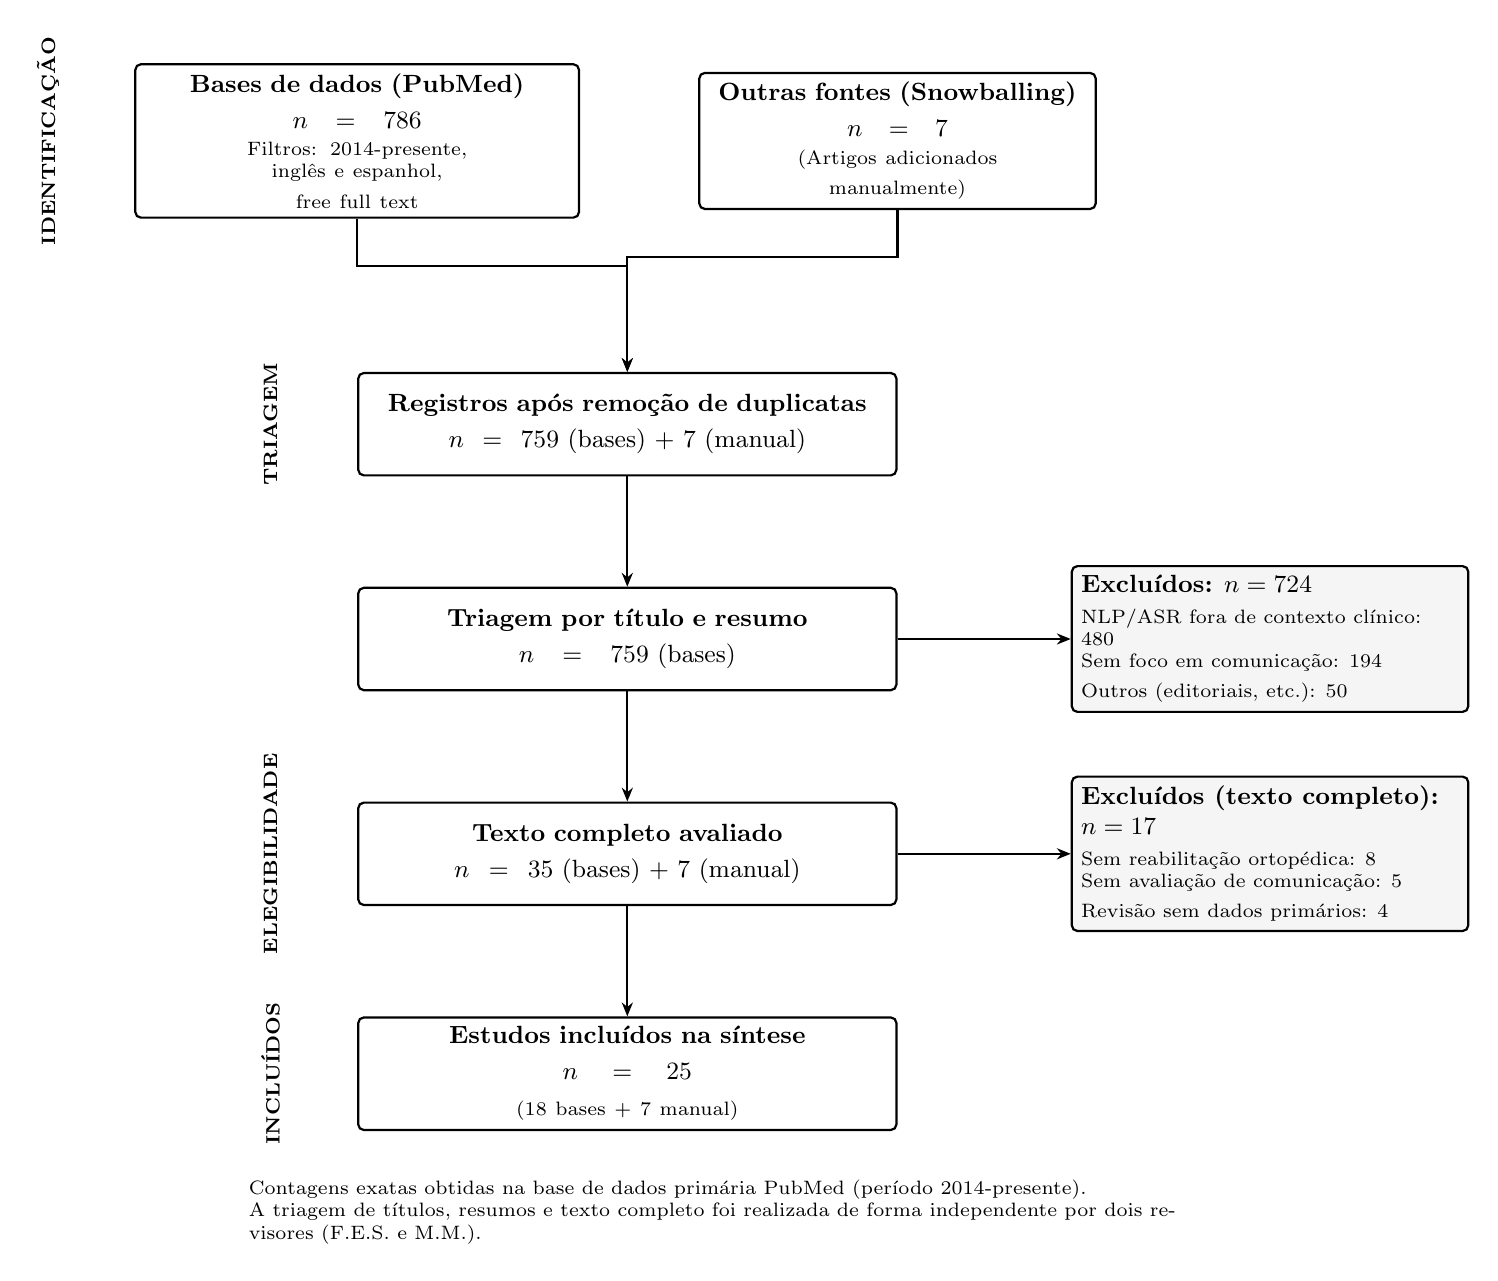
\begin{tikzpicture}[
  %% caixas do fluxo principal
  mbox/.style={
    rectangle, draw=black, thick, rounded corners=2pt,
    minimum width=6.8cm, text width=6.6cm,
    minimum height=1.3cm, align=center,
    fill=white, font=\small
  },
  %% caixas de exclusão (margem direita)
  ebox/.style={
    rectangle, draw=black, thick, rounded corners=2pt,
    minimum width=5.0cm, text width=4.8cm,
    minimum height=1.3cm, align=flush left,
    fill=gray!8, font=\small
  },
  %% setas
  arr/.style={-{Stealth[length=5pt,width=4pt]}, thick},
  %% labels de fase
  phase/.style={font=\bfseries\scriptsize, rotate=90, anchor=center}
]

%% ================================================================
%% ================================================================
%% FASE 1 — IDENTIFICAÇÃO
%% ================================================================
\node[mbox, minimum width=5.6cm, text width=5.4cm] (dbbox) at (-1.8, 0) {
  \textbf{Bases de dados (PubMed)}\\[2pt]
  $n = 786$\\[2pt]
  {\scriptsize Filtros: 2014-presente,\\
    inglês e espanhol,\\
    free full text}
};

\node[mbox, minimum width=5.0cm, text width=4.8cm,
      right=1.5cm of dbbox] (otherbox) {
  \textbf{Outras fontes (Snowballing)}\\[2pt]
  $n = 7$\\[2pt]
  {\scriptsize (Artigos adicionados\\
    manualmente)}
};

%% ================================================================
%% FASE 2 — TRIAGEM
%% ================================================================
%% Centro entre as duas caixas de identificação
\coordinate (midid) at ($(dbbox.south)!0.5!(otherbox.south)$);

\node[mbox, below=2.0cm of midid, anchor=north] (dedup) {
  \textbf{Registros após remoção de duplicatas}\\[2pt]
  $n = 759$ (bases) + $7$ (manual)
};

%% setas de convergência
\draw[arr] (dbbox.south)  -- ++(0,-0.6cm) -| (dedup.north);
\draw[arr] (otherbox.south) -- ++(0,-0.6cm) -| (dedup.north);

\node[mbox, below=1.4cm of dedup] (screen) {
  \textbf{Triagem por título e resumo}\\[2pt]
  $n = 759$ (bases)
};

\draw[arr] (dedup) -- (screen);

\node[ebox, right=2.2cm of screen] (excl1) {
  \textbf{Excluídos:} $n = 724$\\[3pt]
  {\scriptsize
    NLP/ASR fora de contexto clínico: 480\\
    Sem foco em comunicação: 194\\
    Outros (editoriais, etc.): 50
  }
};

\draw[arr] (screen.east) -- (excl1.west);

%% ================================================================
%% FASE 3 — ELEGIBILIDADE
%% ================================================================
\node[mbox, below=1.4cm of screen] (eligib) {
  \textbf{Texto completo avaliado}\\[2pt]
  $n = 35$ (bases) + $7$ (manual)
};

\draw[arr] (screen) -- (eligib);

\node[ebox, right=2.2cm of eligib] (excl2) {
  \textbf{Excluídos (texto completo):} $n = 17$\\[3pt]
  {\scriptsize
    Sem reabilitação ortopédica: 8\\
    Sem avaliação de comunicação: 5\\
    Revisão sem dados primários: 4
  }
};

\draw[arr] (eligib.east) -- (excl2.west);

%% ================================================================
%% FASE 4 — INCLUÍDOS
%% ================================================================
\node[mbox, below=1.4cm of eligib] (included) {
  \textbf{Estudos incluídos na síntese}\\[2pt]
  $n = 25$\\[2pt]
  {\scriptsize (18 bases + 7 manual)}
};

\draw[arr] (eligib) -- (included);

%% ================================================================
%% LABELS DE FASE (margem esquerda)
%% ================================================================
\node[phase] at ($(dbbox.west) + (-1.1cm, 0)$)      {IDENTIFICAÇÃO};
\node[phase] at ($(dedup.west)  + (-1.1cm, 0)$)      {TRIAGEM};
\node[phase] at ($(screen.west) + (-1.1cm, 0)$)      {};   %% continua triagem
\node[phase] at ($(eligib.west) + (-1.1cm, 0)$)      {ELEGIBILIDADE};
\node[phase] at ($(included.west) + (-1.1cm, 0)$)    {INCLUÍDOS};

%% ================================================================
%% NOTA DE RODAPÉ
%% ================================================================
\node[font=\scriptsize, anchor=north west, text width=12cm]
  at ($(included.south west) + (-1.5cm, -0.5cm)$) {%
  Contagens exatas obtidas na base de dados primária PubMed (período 2014-presente). \\
  A triagem de títulos, resumos e texto completo foi realizada de forma independente por dois revisores (F.E.S.\ e M.M.).
};

\end{tikzpicture}